\documentclass[border=2mm,tikz,preview]{standalone}
               
\usetikzlibrary{positioning,chains}

\begin{document}

% Tikz commands based on https://tex.stackexchange.com/a/263761

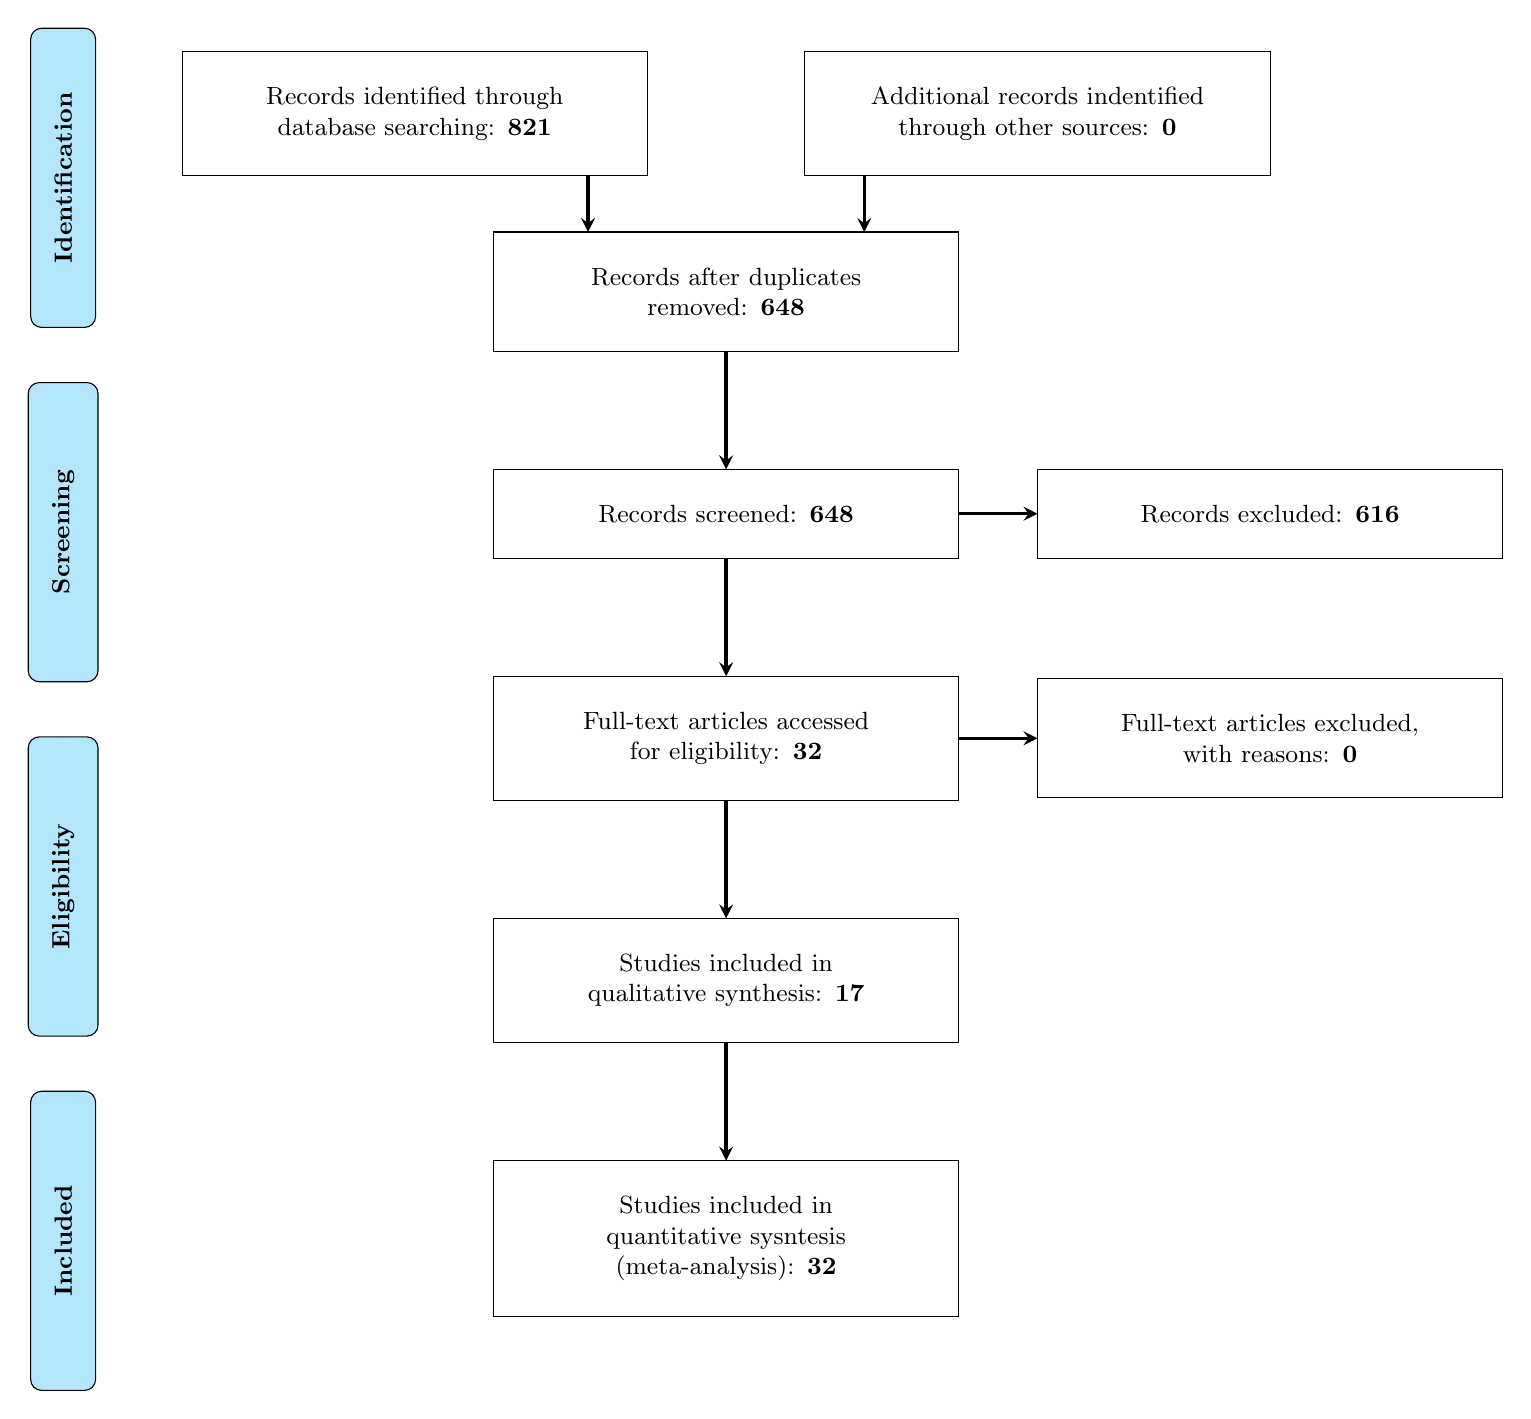
\begin{tikzpicture}[
	node distance=15mm and 10mm,
	start chain=going below,
	mynode/.style = {
		draw, rectangle, align=center, text width=5cm,
		font=\small, inner sep=3ex, outer sep=0pt,
		on chain},
	mylabel/.style = {
		draw, rectangle, align=center, rounded corners, 
		font=\small\bfseries, inner sep=2ex, outer sep=0pt,
		fill=cyan!30, minimum height=38mm,
		on chain},
	every join/.style = arrow,
	arrow/.style = {very thick,-stealth}
]
\coordinate (tc);

%\node[above=of tc,font=\bfseries] {PRISMA 2009 Flow Diagram};

\node (n1a) [mynode, left=of tc]    {Records identified through 
                                     database searching: {\bf 821}};
\node (n1b) [mynode,right=of tc]    {Additional records indentified\\
                                     through other sources: {\bf 0}};

\node (n2)  [mynode, below=of tc]   {Records after duplicates\\
                                     removed: {\bf 648}};
\node (n3)  [mynode,join]   {Records screened: {\bf 648}};
\node (n4)  [mynode,join]   {Full-text articles accessed\\ 
                             for eligibility: {\bf 32}};
\node (n5)  [mynode,join]   {Studies included in \\
                             qualitative synthesis: {\bf 17}};
\node (n6)  [mynode,join]   {Studies included in \\
                             quantitative sysntesis\\
                                (meta-analysis): {\bf 32}};

\node (n3r) [mynode,right=of n3]    {Records excluded: {\bf 616}};
\node (n4r) [mynode,right=of n4]    {Full-text articles excluded,\\
                                        with reasons: {\bf 0}};
                                    
\draw[arrow] ([xshift=+22mm] n1a.south) coordinate (a)
                                       -- (a |- n2.north);
\draw[arrow] ([xshift=-22mm] n1b.south) coordinate (b)
                                       -- (b |- n2.north);
\draw[arrow] (n3) -- (n3r);
\draw[arrow] (n4) -- (n4r);

	\begin{scope}[node distance=7mm]
		\node[mylabel,below left=-3mm and 11mm of n1a.north west]
						{\rotatebox{90}{Identification}};
		\node[mylabel]  {\rotatebox{90}{Screening}};
		\node[mylabel]  {\rotatebox{90}{Eligibility}};
		\node[mylabel]  {\rotatebox{90}{Included}};
	\end{scope}
\end{tikzpicture}

\end{document}
